\model{Ragged Array}

\jafile{Ragged.java}

\begin{center}
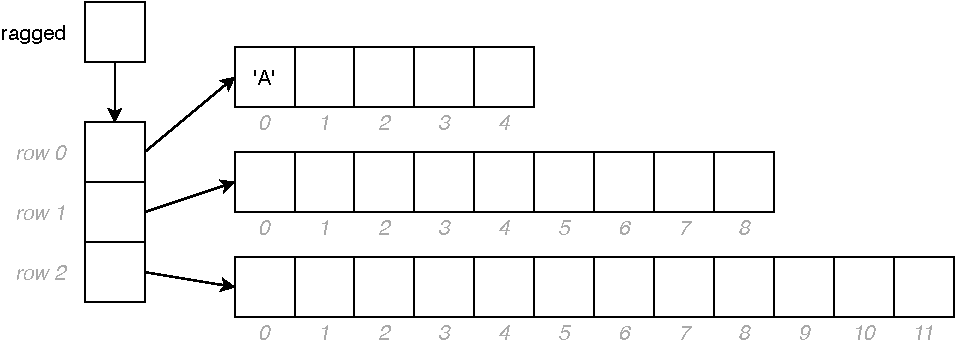
\includegraphics[scale=0.92]{RaggedArray.pdf}
\end{center}


\quest{20 min}


\Q Based on the \java{main} method above:

\setlength{\defaultwidth}{3em}

\begin{enumerate}
\item How many rows are in this 2D array?     \ans{3}
\item How many columns are in the first row?  \ans{5}
\item How many columns are in the second row? \ans{9}
\item How many columns are in the third row?  \ans{12}
\end{enumerate}

\vspace{-1ex}


\Q Run the program. What is the value of \java{letter} at the end? \ans{\chr{B}}

\vspace{1ex}


\Q Describe what happens when you increment a \java{char} variable.

\begin{answer}[3em]
The next letter in the (Unicode) alphabet is assigned.

\medskip
Note: Characters in Java are represented by 16-bit integers.
\end{answer}


\Q Summarize the main difference in shape between the ``rectangular'' array of \ref{model1.tex} and the ``ragged'' array of \ref{model2.tex}.

\begin{answer}[3em]
Rectangular arrays have the same number of columns on each row.
Ragged arrays do not.
\end{answer}


%\Q Identify the difference between how the ``rectangular'' array of \ref{model1.tex} and the ``ragged'' array of \ref{model2.tex} were created.
%
%\begin{answer}
%The rectangular array was created using array initializers, e.g., \java{\{1, 2, 3\}}.
%The ragged array was created using the \jans{new} keyword to instantiate each row.
%\end{answer}


\Q Examine your code for Question \ref{key1}.
Would it work for the \java{ragged} array?
Explain why or why not.

\begin{answer}[3em]
It would still work, because the inner loop processes only the number of elements in that particular row.
\end{answer}


\Q \label{key3}
Complete the following steps to fill the contents of the \java{ragged} array:

\begin{enumerate}
\item Copy your code from Question \ref{key1} and paste it in Model2.java at the end of the main method.
Replace the variable \java{table} with \java{ragged} so that it compiles.

\item Comment out lines 9--11 so that \java{letter} is not modified and printed before the first loop.

\item Modify your code so that it sets the first element of \java{ragged} to \chr{A}, the second element to \chr{B}, and so on, until the last element is set to \chr{Z}.
(Hint: Move lines 9--10 into the loop.)

\item Copy your code from Question \ref{key1} again and paste it in Model2.java at the end of the main method. Run the program to verify that all letters were set correctly.

\item Paste your code from step c) in the space below:
\end{enumerate}

\begin{answer}[9em]
\begin{javaans}
for (int row = 0; row < ragged.length; row++) {
    for (int col = 0; col < ragged[row].length; col++) {
        ragged[row][col] = letter;
        letter++;
    }
}
\end{javaans}
\end{answer}


\Q Which kind of 2D array (rectangular or ragged) would you use to represent the lanes of a highway, where the array elements are car objects? Justify your answer.

\begin{answer}[3em]
A ragged array, because there could be a different number of cars in each lane of the highway.
\end{answer}


\Q Which kind of 2D array (rectangular or ragged) would you use to represent a matrix in mathematics, where the array elements are integers? Justify your answer.

\begin{answer}[3em]
A rectangular array, because matrices have the same number of columns on each row.
\end{answer}
